% !TEX TS-program = pdflatex
% !TEX root = ../tesi.tex

\chapter{Conclusioni}
Il progetto di ricerca realizzato da CIBRA e Nauta ha impiegato 3 giorni di registrazioni, in concomitanza con condizioni meteo avverse e non. 
Sono stati poi deposti altri 3 registratori durante le giornate nella zona di San Foca, e poi il loro recupero con annesso controllo delle registrazioni.
Con un totale di 100 miglia nautiche in mare, 25 ore 40 minuti in mare. 

\begin{figure}[h]
\centering
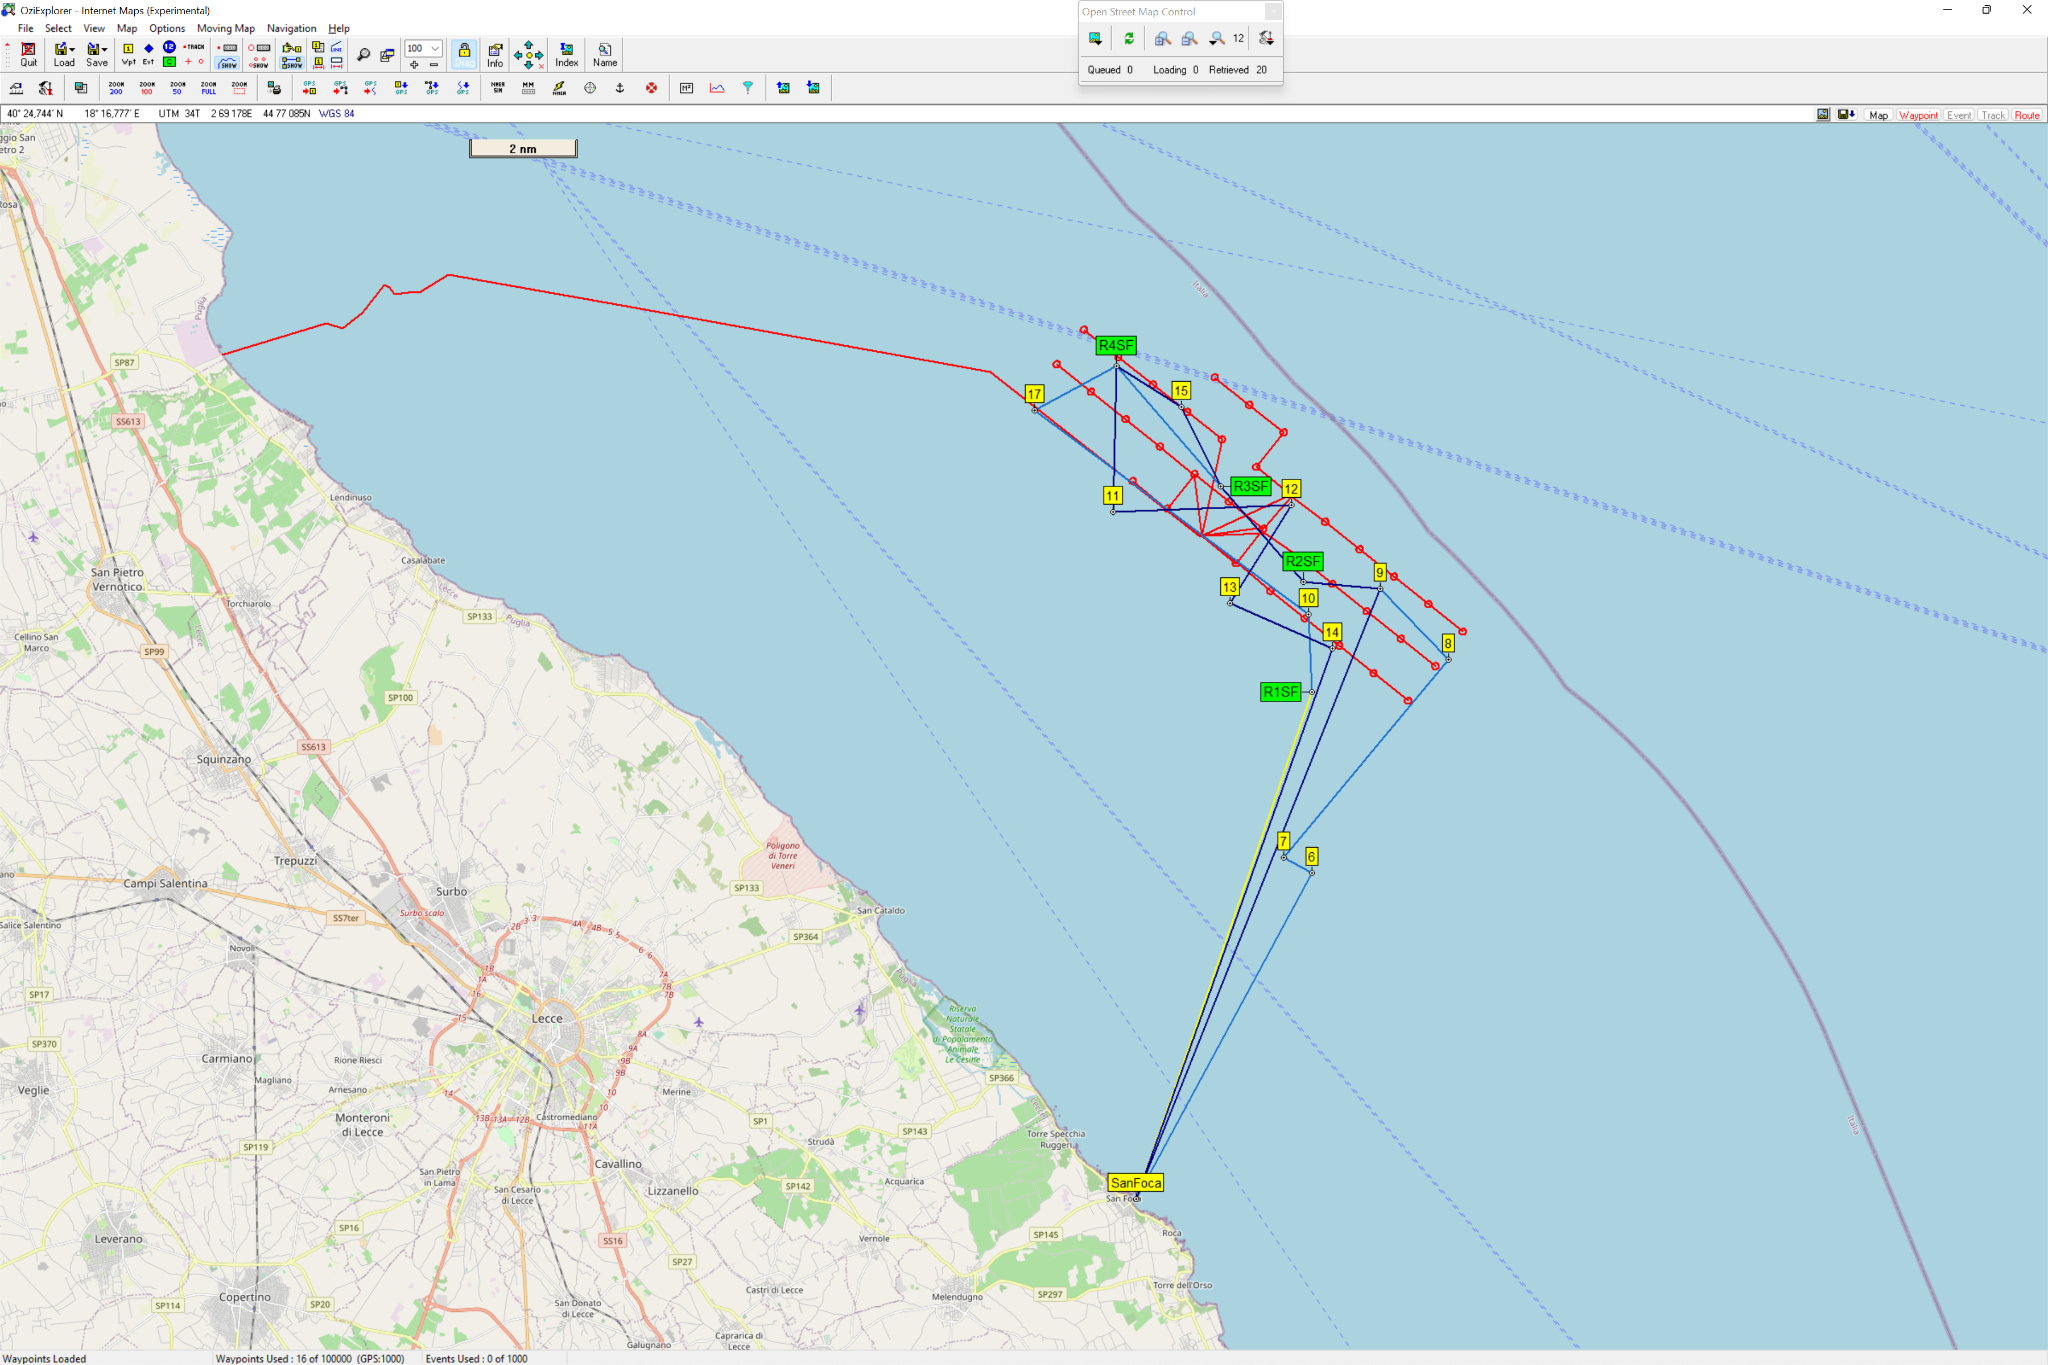
\includegraphics[width=.45\textwidth]{mappa-con-i-percorsi-di-registrazione}
\caption{Mappa con i percorsi impostati nelle tre giornate e le stazioni acustiche. In rosso i punti dell’impianto in progetto}
\end{figure}

I risultati riportati nella sezione precedente dimostrano chiaramente come l’area in oggetto sia estremamente rumorosa.
Le analisi dei file acustici hanno evidenziato come questa rumorosità sia direttamente legata al traffico marittimo presente. 
In questo contesto ampiamente compromesso, dove i livelli di rumore risultano molto più elevati che in altre aree del mar Adriatico, l’apporto del campo eolico in fase operativa è verosimilmente trascurabile. 
Il modello di previsione dell’impatto acustico dell’opera ha comportato, a livello di impostazione, alcune difficoltà. 
Le conoscenze e le misure associate ai campi eolici galleggianti e le relative misurazioni in campo sono infatti ancora lacunose, data la relativamente giovane età di tale tipo di installazione con questi valori di potenza. 
La tecnologia nel settore avanza rapidamente, e le turbine in programma di messa in opera in questo progetto sono al momento solo in fase di prototipo. 
I dati di riferimento per l’esecuzione del modello derivano quindi da misure effettuate in installazioni simili e scalate in termini di potenza e numero di torri. 
Questa assunzione, unica via al momento percorribile, potrebbe non essere del tutto corrispondente alla realtà. 

Grazie al Dott. Claudio Fossati, Dott. Michele Manghi Dott. Gianni Pavan, e al lavoro di ricerca effettuato circa 2 anni fa, aiuterà oggi a capire come la nostra natura possa essere tutelata e preservata dalla mano dell'uomo. 
Non di minore importante sono stati e saranno ancora lo sviluppo di strumenti più completi in questo campo per la scoperta di quanto l'inquinamento acustico possa essere compromettente per tutto l'ambiente marino e non. 

La Legge Quadro n.447/1995, nello stabilire i principi fondamentali in materia di tutela dell'ambiente esterno e dell'ambiente abitativo dall'inquinamento acustico, introduce valori limite di emissione, di immissioneassoluti e differenziali, 
di attenzione, di qualità, valori di immissione specifico secondo le definizioni di seguito riportate:
\begin{itemize}
\item - valori limite di emissione: il valore massimo di rumore che può essere emesso da una sorgente sonora, misurato in prossimità della sorgente stessa;
\item - valori limite di immissione: il valore massimo di rumore che può essere immesso da una o più sorgenti sonore nell'ambiente abitativo o nell'ambiente esterno, misurato in prossimità dei ricettori. 
\end{itemize}

I valori limite di immissione sono distinti in:
\begin{itemize}
\item a) valori limite assoluti, determinati con riferimento al livello equivalente di rumore ambientale;
\item b) valori limite differenziali, determinati con riferimento alla differenza tra il livello equivalente di rumore ambientale ed il rumore residuo;
\end{itemize}

\begin{itemize}
\item - valore di attenzione: il valore di immissione, indipendente dalla tipologia della sorgente e dalla classificazione acustica del territorio della zona da proteggere, il cui superamento obbliga ad un intervento di mitigazione acustica e rende applicabili, laddove
ricorrono i presupposti, speciali forme di contenimento o di abbattimento delle emissioni sonore, disposte con provvedimento motivato dalle competenti autorità (L.Q. n.447/95, art.9);
\item - valori di qualità: i valori di rumore da conseguire nel breve, nel medio e nel lungo periodo con le tecnologie e le metodiche di risanamento disponibili, per realizzare gli obiettivi di tutela previsti dalla legge;
\item- valore limite di immissione specifico: valore massimo del contributo della sorgente sonora specifica misurato in ambiente esterno ovvero in facciata al ricettore.

È necessario precisare che, ad oggi, non sono stati numericamente fissati e, pertanto, non risultano applicabili né il valore limite di immissione specifico, né il valore di attenzione, come definito a seguito della modifica normativa introdotta dal D.Lgs. n.42/2017.
Al proposito, è indispensabile sottolineare che, a seguito di tale modifica, si è venuta a creare una criticità, che auspicabilmente potrà essere risolta nell'ambito dei lavori di revisione dei decreti vigenti, in relazione alla mancata contestuale modifica dell’articolo 7 della L.Q. n.
447/1995: ad oggi, i Comuni continuano, da un punto di vista formale, ad avere l'obbligo di adottare un piano di risanamento  e/o in caso di superamento dei valori di attenzione.
I decreti attuativi della Legge Quadro hanno in seguito delineato una complessa architettura legislativa, tuttora non completata, che definisce gli ambiti di applicazione e le modalità di misura dei valori limite vigenti.


